\documentclass[10pt,a4paper,onecolumn]{article}
% \usepackage[utf8]{inputenc}
\usepackage{marginnote}
\usepackage{graphicx}
\usepackage{xcolor}
\usepackage{authblk,etoolbox}
\usepackage{amssymb,amsmath}
\usepackage{titlesec}
\usepackage{calc}
\usepackage{hyperref}
\hypersetup{breaklinks=true,
            bookmarks=true,
            pdfauthor=
{
      Dominique Caron,
      Vincent Lessard,
      Qile Wu,
      Timothée Poisot,
  },
            pdftitle=
{
[Re] Insect natural enemies as regulating factors
},
            colorlinks=true,
            citecolor=blue,
            urlcolor=blue,
            linkcolor=blue,
            pdfborder={0 0 0}}
\urlstyle{same}
\usepackage{tcolorbox}
\usepackage{ragged2e}
\usepackage{fontspec}
\usepackage{fontawesome}
\usepackage{caption}
\usepackage{listings}
\lstnewenvironment{code}{\lstset{language=Haskell,basicstyle=\small\ttfamily}}{}



%\usepackage{fancyvrb}
%\VerbatimFootnotes
%\usepackage{graphicx}
%\usepackage{mdframed}
%\newmdenv[backgroundcolor=lightgray]{Shaded}


\usepackage{longtable,booktabs}

\usepackage[
  backend=biber,
%  style=alphabetic,
%  citestyle=numeric
]{biblatex}
\bibliography{bibliography.bib}



% --- Macros ------------------------------------------------------------------
\renewcommand*{\bibfont}{\small \sffamily}

\definecolor{red}{HTML}{CF232B}
\newcommand{\ReScience}{Re{\bfseries \textcolor{red}{Science}}}

\newtcolorbox{rebox}
   {colback=blue!5!white, colframe=blue!40!white,
     boxrule=0.5pt, arc=2pt, fonttitle=\sffamily\scshape\bfseries,
     left=6pt, right=20pt, top=6pt, bottom=6pt}

\newtcolorbox{repobox}
   {colback=red, colframe=red!75!black,
     boxrule=0.5pt, arc=2pt, left=6pt, right=6pt, top=3pt, bottom=3pt}

% fix for pandoc 1.14
\newcommand{\tightlist}{%
  \setlength{\itemsep}{1pt}\setlength{\parskip}{0pt}\setlength{\parsep}{0pt}}

% --- Style -------------------------------------------------------------------
\renewcommand*{\bibfont}{\small \sffamily}
\renewcommand{\captionfont}{\small\sffamily}
\renewcommand{\captionlabelfont}{\bfseries}

\makeatletter
\renewcommand\@biblabel[1]{{\bf #1.}}
\makeatother

% --- Page layout -------------------------------------------------------------
\usepackage[top=3.5cm, bottom=3cm, right=1.5cm, left=1.5cm,
            headheight=2.2cm, reversemp, includemp, marginparwidth=4.5cm]{geometry}

% --- Section/SubSection/SubSubSection ----------------------------------------
\titleformat{\section}
  {\normalfont\sffamily\Large\bfseries}
  {}{0pt}{}
\titleformat{\subsection}
  {\normalfont\sffamily\large\bfseries}
  {}{0pt}{}
\titleformat{\subsubsection}
  {\normalfont\sffamily\bfseries}
  {}{0pt}{}
\titleformat*{\paragraph}
  {\sffamily\normalsize}


% --- Header / Footer ---------------------------------------------------------
\usepackage{fancyhdr}
\pagestyle{fancy}
%\renewcommand{\headrulewidth}{0.50pt}
\renewcommand{\headrulewidth}{0pt}
\fancyhead[L]{\hspace{-1cm}\includegraphics[width=4.0cm]{rescience-logo.pdf}}
\fancyhead[C]{}
\fancyhead[R]{}
\renewcommand{\footrulewidth}{0.25pt}

\fancyfoot[L]{\hypersetup{urlcolor=red}
              \sffamily \ReScience~$\vert$
              \href{http://rescience.github.io}{rescience.github.io}
              \hypersetup{urlcolor=blue}}
\fancyfoot[C]{\sffamily 1 - \thepage}
\fancyfoot[R]{\sffamily Sep 2015 $\vert$
                        Volume \textbf{1} $\vert$
                        Issue \textbf{1}}
\pagestyle{fancy}
\makeatletter
\let\ps@plain\ps@fancy
\fancyheadoffset[L]{4.5cm}
\fancyfootoffset[L]{4.5cm}

% --- Title / Authors ---------------------------------------------------------
% patch \maketitle so that it doesn't center
\patchcmd{\@maketitle}{center}{flushleft}{}{}
\patchcmd{\@maketitle}{center}{flushleft}{}{}
% patch \maketitle so that the font size for the title is normal
\patchcmd{\@maketitle}{\LARGE}{\LARGE\sffamily}{}{}
% patch the patch by authblk so that the author block is flush left
\def\maketitle{{%
  \renewenvironment{tabular}[2][]
    {\begin{flushleft}}
    {\end{flushleft}}
  \AB@maketitle}}
\makeatletter
\renewcommand\AB@affilsepx{ \protect\Affilfont}
%\renewcommand\AB@affilnote[1]{{\bfseries #1}\hspace{2pt}}
\renewcommand\AB@affilnote[1]{{\bfseries #1}\hspace{3pt}}
\makeatother
\renewcommand\Authfont{\sffamily\bfseries}
\renewcommand\Affilfont{\sffamily\small\mdseries}
\setlength{\affilsep}{1em}

\LetLtxMacro{\OldIncludegraphics}{\includegraphics}
\renewcommand{\includegraphics}[2][]{\OldIncludegraphics[width=12cm, #1]{#2}}


% --- Document ----------------------------------------------------------------
\title{[Re] Insect natural enemies as regulating factors}

    \usepackage{authblk}
                        \author[1]{Dominique Caron}
                    \author[1]{Vincent Lessard}
                    \author[1]{Qile Wu}
                    \author[1]{Timothée Poisot}
                            \affil[1]{Département de sciences biologiques, Université de Montréal, Montréal,
Québec, Canada}
                    \affil[2]{Québec Centre for Biodiversity Sciences, Montréal, Québec, Canada}
            
\date{\vspace{-5mm}
      \sffamily \small \href{mailto:timothee.poisot@umontreal.ca}{timothee.poisot@umontreal.ca}}


\setlength\LTleft{0pt}
\setlength\LTright{0pt}


\begin{document}
\maketitle

\marginpar{
  %\hrule
  \sffamily\small
  %\vspace{2mm}
  {\bfseries Editor}\\
  Name Surname\\

  {\bfseries Reviewers}\\
        Name Surname\\
        Name Surname\\
  
  {\bfseries Received}  Sep, 1, 2015\\
  {\bfseries Accepted}  Sep, 1, 2015\\
  {\bfseries Published} Sep, 1, 2015\\

  {\bfseries Licence}   \href{http://creativecommons.org/licenses/by/4.0/}{CC-BY}

  \begin{flushleft}
  {\bfseries Competing Interests:}\\
  The authors have declared that no competing interests exist.
  \end{flushleft}

  \hrule
  \vspace{3mm}

  \hypersetup{urlcolor=white}

    \vspace{-1mm}
  \begin{repobox}
    \bfseries\normalsize
      \href{https://github.com/BIO6032/2018\_replication\_hassell\_1985/article}{\faGithubAlt~Article repository}
  \end{repobox}
      \vspace{-1mm}
  \begin{repobox}
    \bfseries\normalsize
      \href{https://github.com/BIO6032/2018\_replication\_hassell\_1985/code}{\faGithubAlt~Code repository}
  \end{repobox}
        \hypersetup{urlcolor=blue}
}

\begin{rebox}
\sffamily {\bfseries A reference implementation of}
\small
\begin{flushleft}
\begin{itemize}
    \item[→] Hassell, M. P. Insect Natural Enemies as Regulating Factors. Journal of
Animal Ecology, vol.~54, no. 1, 1985, pp.~323--334.
  \end{itemize}\par
\end{flushleft}
\end{rebox}


\hypertarget{introduction}{%
\section{Introduction}\label{introduction}}

Parasitism is a special case of predation. In both interactions, a
species (parasitoid or predator) feeds on the other species (host or
prey), acting as a regulating factor (\textcite{Anderson78}). However,
the population dynamics of both systems are very different.
\textcite{Thompson24} was the first to propose a model to describe this
host-parasitoid system. In his model, parasites are limited by the
number of eggs they lay. Depending on the relative increase rate of
hosts and parasites, either both population increase indefinitely or
decrease to extinction. Later, \textcite{Nicholson35} proposed other
models for which the rate of increase of the parasites is limited by
their capacity to find hosts. These were the basis for many other models
where parasites act as regulating factors (\textcite{Hassell78};
\textcite{Rockwood15}).

In 1983, \textcite{Dempster83} proposed that natural enemies may not be
an important regulating factor in insect dynamics. In fact, he failed to
detect density-dependence due to natural enemies in most of the studies
on Lepidoptera he reviewed. His proposition really contrasted with what
was thought at the time. In response to this article,
\textcite{Hassell85} analyzed an insect dynamic model in which the only
regulating factor was natural enemies. He showed that the difficulties
to detect the density-dependent effect of natural enemies was due to
time delays and stochasticity. This paper is still considered a classic
in fields of insect and host-parasitoid population dynamics. It
introduced an important argument on the role of natural enemies on
insect populations, a controversial topic that aroused ecologists to
debate for almost a decade (\textcite{Turchin90}).

We used information from \textcite{Hassell85} to replicate the model. We
were able to replicate the results central to the article. In addition,
we made new analyses for the stochastic models that bring additional
support to \textcite{Hassell85} arguments. To our best knowledge, the
original implementation was not available. The code for the simulations
and the figures were written in \emph{Julia} v0.6.2.

\hypertarget{methods}{%
\section{Methods}\label{methods}}

The mathematical formulation used in this paper to show the difficulties
of detecting natural enemies as regulating factors are the same that
were used in the original paper by \textcite{Hassell85} . First of all,
the host population dynamics are given as

\begin{equation}N_{t+1} = F \times N_t \times f(N_t,P_t) \times D\label{eq:1}\end{equation}

where \(N_t\) and \(N_{t+1}\) represent the host population at
generation \(t\) and at the next generation, \(F\) is the rate of
increase of the population and \(D\) is the density independent
probability of survival of the hosts (mortality). The specialist
parasitoids population dynamics are represented by

\begin{equation}P_{t+1} = c \times N_t \times [1-f(N_t, P_t)]\label{eq:2}\end{equation}

where \(P_t\) and \(P_{t+1}\) are the number of parasitoids at
generation \(t\) and at the next one, while \(c\) is the number of
female parasitoids emerging from each host parasitized. In both
eq.~\ref{eq:1} and eq.~\ref{eq:2}, \(f(N_t,P_t)\) represents the
probability of escaping mortality from natural enemies (parasitoids) and
is given by eq.~\ref{eq:3}.

\begin{equation}f(N_t,P_t) = [1 + (a \times P_t) / (m \times (1 + a \times T_h \times N_t))]^{-m} \label{eq:3}\end{equation}

where \(a\) is the per capita searching efficiency of the parasitoids,
\(m\) is the extent of clumping of the parasitoids attacks and \(T_h\)
is the handling time as a proportion of the total time. This paper also
explores the relationship between the hosts and a generalist parasitoid
population. Generalist parasite dynamics follows the equation

\begin{equation}P_t = h \times \left(1 - \text{exp}\left(-\frac{N_t}{b}\right)\right)\label{eq:4}\end{equation}

where \(h\) is the saturation number of parasitoids and \(b\) is the
rate of approaching this saturation number.

To determine if the natural enemies can be declared as density-dependent
factors, the host population mortality due to parasitism (\(k-value\))
is plotted against population density for each simulated generation. The
correlation coefficient \(r\) of the resulting scatter plot indicates
the strength of the density-dependence of natural enemies. The higher
\(r\) is, the strongest the relation between hosts and parasites is. The
host mortality is given by

\begin{equation}k_\text{value} = \text{log}_{10}\frac{N_t}{S}\label{eq:5}\end{equation}

where \(S\) is the number of hosts that survived parasitism. This number
is given by the host population density multiplied by the probability of
escaping mortality from natural enemies (eq.~\ref{eq:6}).

\begin{equation}S = N_t \times f(N_t,P_t)\label{eq:6}\end{equation}

The objective in this paper is to reproduce the main results of the
original publication. Therefore, we did not reproduce figures 1, 2 and
7. Figure 1 was a schematic representation of an insect life cycle.
Figure 2 and Figure 7 represent relationship between parameters and
population size/proportion of parasited host. Therefore, they are not
necessary in order to show how difficult it is to detect the regulating
effect of natural enemies on a host population. For every figure
reproduced, we used the exact same values that were used in the original
paper for the different parameters.

The software used to code and run the models and to generate the figures
is \emph{Julia} version 0.6.2 (\textcite{Bezanson17}) All the code used
to replicate the original paper is available alongside the article.

\hypertarget{results}{%
\section{Results}\label{results}}

\hypertarget{deterministic-model}{%
\subsubsection{Deterministic model}\label{deterministic-model}}

The reproduced population dynamics for the host population and for the
specialist parasitoids (fig.~\ref{fig:figure3} (a) and (b)) are very
similar to the ones in Hassell's paper. When the level of clumping of
parasitoid attacks is high, both populations decrease during the first
10 generations before they stabilize, with the host population twice as
big as the specialist parasitoid population. When the extent of clumping
is lower, both populations show decreasing oscillations during the 50
simulated generations. The difference between this article and the
original publication resides in the fig.~\ref{fig:figure3} (c) and (d),
where we standardized the axes of the graphs. At first sight, in
Hassell's paper, the \(k-values\) in fig.~\ref{fig:figure3} (c) seem
almost as high as in fig.~\ref{fig:figure3} (d). However, when using the
same scale for the two graphs, we can see that the \(k-values\) in the
case of high level of clumping show a lot less variation than with a
lower level of clumping.

The simulations performed to study the relationship between the
population dynamics of the hosts and the generalist parasitoids are also
very similar to the ones done by Hassell (fig.~\ref{fig:figure4}). This
shows a density dependant relationship between the two populations,
where the natural enemy regulates the host population until they both
reach a stable equilibrium. This is also the conclusion when we observe
the relation between the two populations in fig.~\ref{fig:figure3} (a)
and (c).

\hypertarget{stochastic-model}{%
\subsubsection{Stochastic model}\label{stochastic-model}}

When the models include stochasticity, the resulting population dynamics
between hosts and parasites are very different compared to the
deterministic models. Overall, the results obtained in the replications
are very similar to the original paper. Whether we look at the model for
the specialist parasitoids or the one for the generalist parasitoids,
both show irregular oscillations in the host-parasitoid population
dynamics (fig.~\ref{fig:figure5} and fig.~\ref{fig:figure6}, (a), (b)
and (c)). The addition of stochastic parameters prevents the
stabilization of host populations and makes it more difficult to
identify parasitoids as a density-dependent control factor, except in
fig.~\ref{fig:figure6} (a). The relationships between the \(k-values\)
and the host density are similar in Hassell's publication and in ours.
However, the regression for these relationships in our replication tend
to have a determination coefficient (\(R^2\)) higher than the one found
by Hassell, but they are generally really close. Discrepancies in the
coefficient of determination can be explained by different routines for
pseudo random number generation.

Moreover, the oscillations we obtained in fig.~\ref{fig:figure6} (b) are
not the same range compared to the original paper. More precisely, the
oscillations we obtained with \(h\) stochastic are smaller compared to
the original paper (fig.~\ref{fig:figure6} (b)).

Because the inclusion of stochastic parameters in the population
dynamics causes variability in the outputs, the results from two
successive simulations can be very different. In order to account for
this variability and to show how it can affect the population dynamics
of the hosts and parasites, we added fig.~\ref{fig:figure7} and
fig.~\ref{fig:figure8}. These figures show the extent of the variation
of the correlation coefficient (\(r\)) obtained in 5000 different
simulations (as opposed to a single simulation in the original article).
A dotted line was added to represent the value of the correlation
coefficient (\(r\)) that came out of the deterministic models. The
values of \(r\) vary greatly for every stochastic parameter. In every
case, the mean value of \(r\) is lower in the stochastic models than in
the deterministic models. This is in agreement with Hassell's results,
and shows that stochasticity makes it harder to detect the density
dependence effect of the parasites, whether they are generalist or
specialist.

\hypertarget{discussion}{%
\section{Discussion}\label{discussion}}

Overall, we were able to replicate most results from
\textcite{Hassell85}. We found the exact same results for the
deterministic model. We standardized the limits for the axes, which was
not the case in the original paper. This allows a more convenient
comparison of the different results.

As expected, we did not find the exact same dynamic for the stochastic
model. The figures we added (fig.~\ref{fig:figure7} and
fig.~\ref{fig:figure8}) showed how adding stochasticity into the model
can cause great variability in the output. For example, in the
specialist parasitoid model with a stochastic density-dependent host
survival (\(D\)), the correlation we found (fig.~\ref{fig:figure7} (a))
was sometimes very weak (\(r \approx 0.2\)) and some other times almost
as strong as the deterministic model (\(r \approx 0.7\)). Also, the
correlation between the mortality from parasitism (\(k\)-value) and host
density (\(N\)) found in the stochastic model was almost always weaker
than in the deterministic model (fig.~\ref{fig:figure7} and
fig.~\ref{fig:figure8}). Therefore, the results we added strongly
support the main argument from the original paper: adding stochasticity
almost always obscures the density-dependent effect of natural enemies.

The discrepancies we noted in the dynamics of the stochastic model with
the generalist parasite and a stochastic saturation number of parasitoid
(\(h\); in fig.~\ref{fig:figure6} (b)) are difficult to explain. It
seems unlikely that it is caused by either our implementation of the
model, or by errors during runtime, since we successfully replicated
results from all the other numerical experiments. Without the original
implementation, we can only speculate on the difference between the
original implementation and ours. This combination of parameters is the
only one with a stochastic parameter normally distributed with a mean
not equal to its associated standard deviation. We tried with an \(h\)
normally distributed with a mean and a standard deviation of 5
(fig.~\ref{fig:figure9}), and the results were a lot more similar to the
one from \textcite{Hassell85} than what we originally had
(fig.~\ref{fig:figure6} (b)). Again, this is only an hypothesis on the
kind of error that could explain the differences between the original
paper and ours. Other possible sources of error include the
pseudo-random numbers generator used, errors in the original
implementation, or errors in the parameter values reported in the
original publication; sadly, these are virtually impossible to rule out.

The mathematical model from the original paper was well detailed, which
allowed us to create our own implementation. The equation for the number
of survivors from parasitism (\(S\)) was the only one we needed to
deduce from our own interpretation. This variable is used in the
computation of the mortality (\(k_\text{value}\)) which is a well
documented index. Therefore, this has not limited us in the replication
of the article, and the fact that the deterministic simulations match
these of the original paper suggests that we used the same formulation
for \(S\).

\hypertarget{conclusion}{%
\section{Conclusion}\label{conclusion}}

We were able to replicate the original results. Even if we did not find
the exact same dynamics for the stochastic models, we draw the same
conclusions : the density-dependent effect from natural enemies is
obscured by time delays and/or stochasticity. This makes it very
difficult to detect natural enemies as regulating factors from life
table data. In addition, we added density plots for the correlation
coefficient from 5000 iterations of each stochastic model. This allowed
us to determine that the differences between our results and Hassell's
were explained by the stochasticity of the models. Also, these new
results add a strong support to the arguments of the original paper. To
conclude, the reproduction of the reference article \textcite{Hassell85}
was successful and we hope it adds to the legacy left by this
significant paper in the history of population dynamics.

\begin{figure}
\hypertarget{fig:figure3}{%
\centering
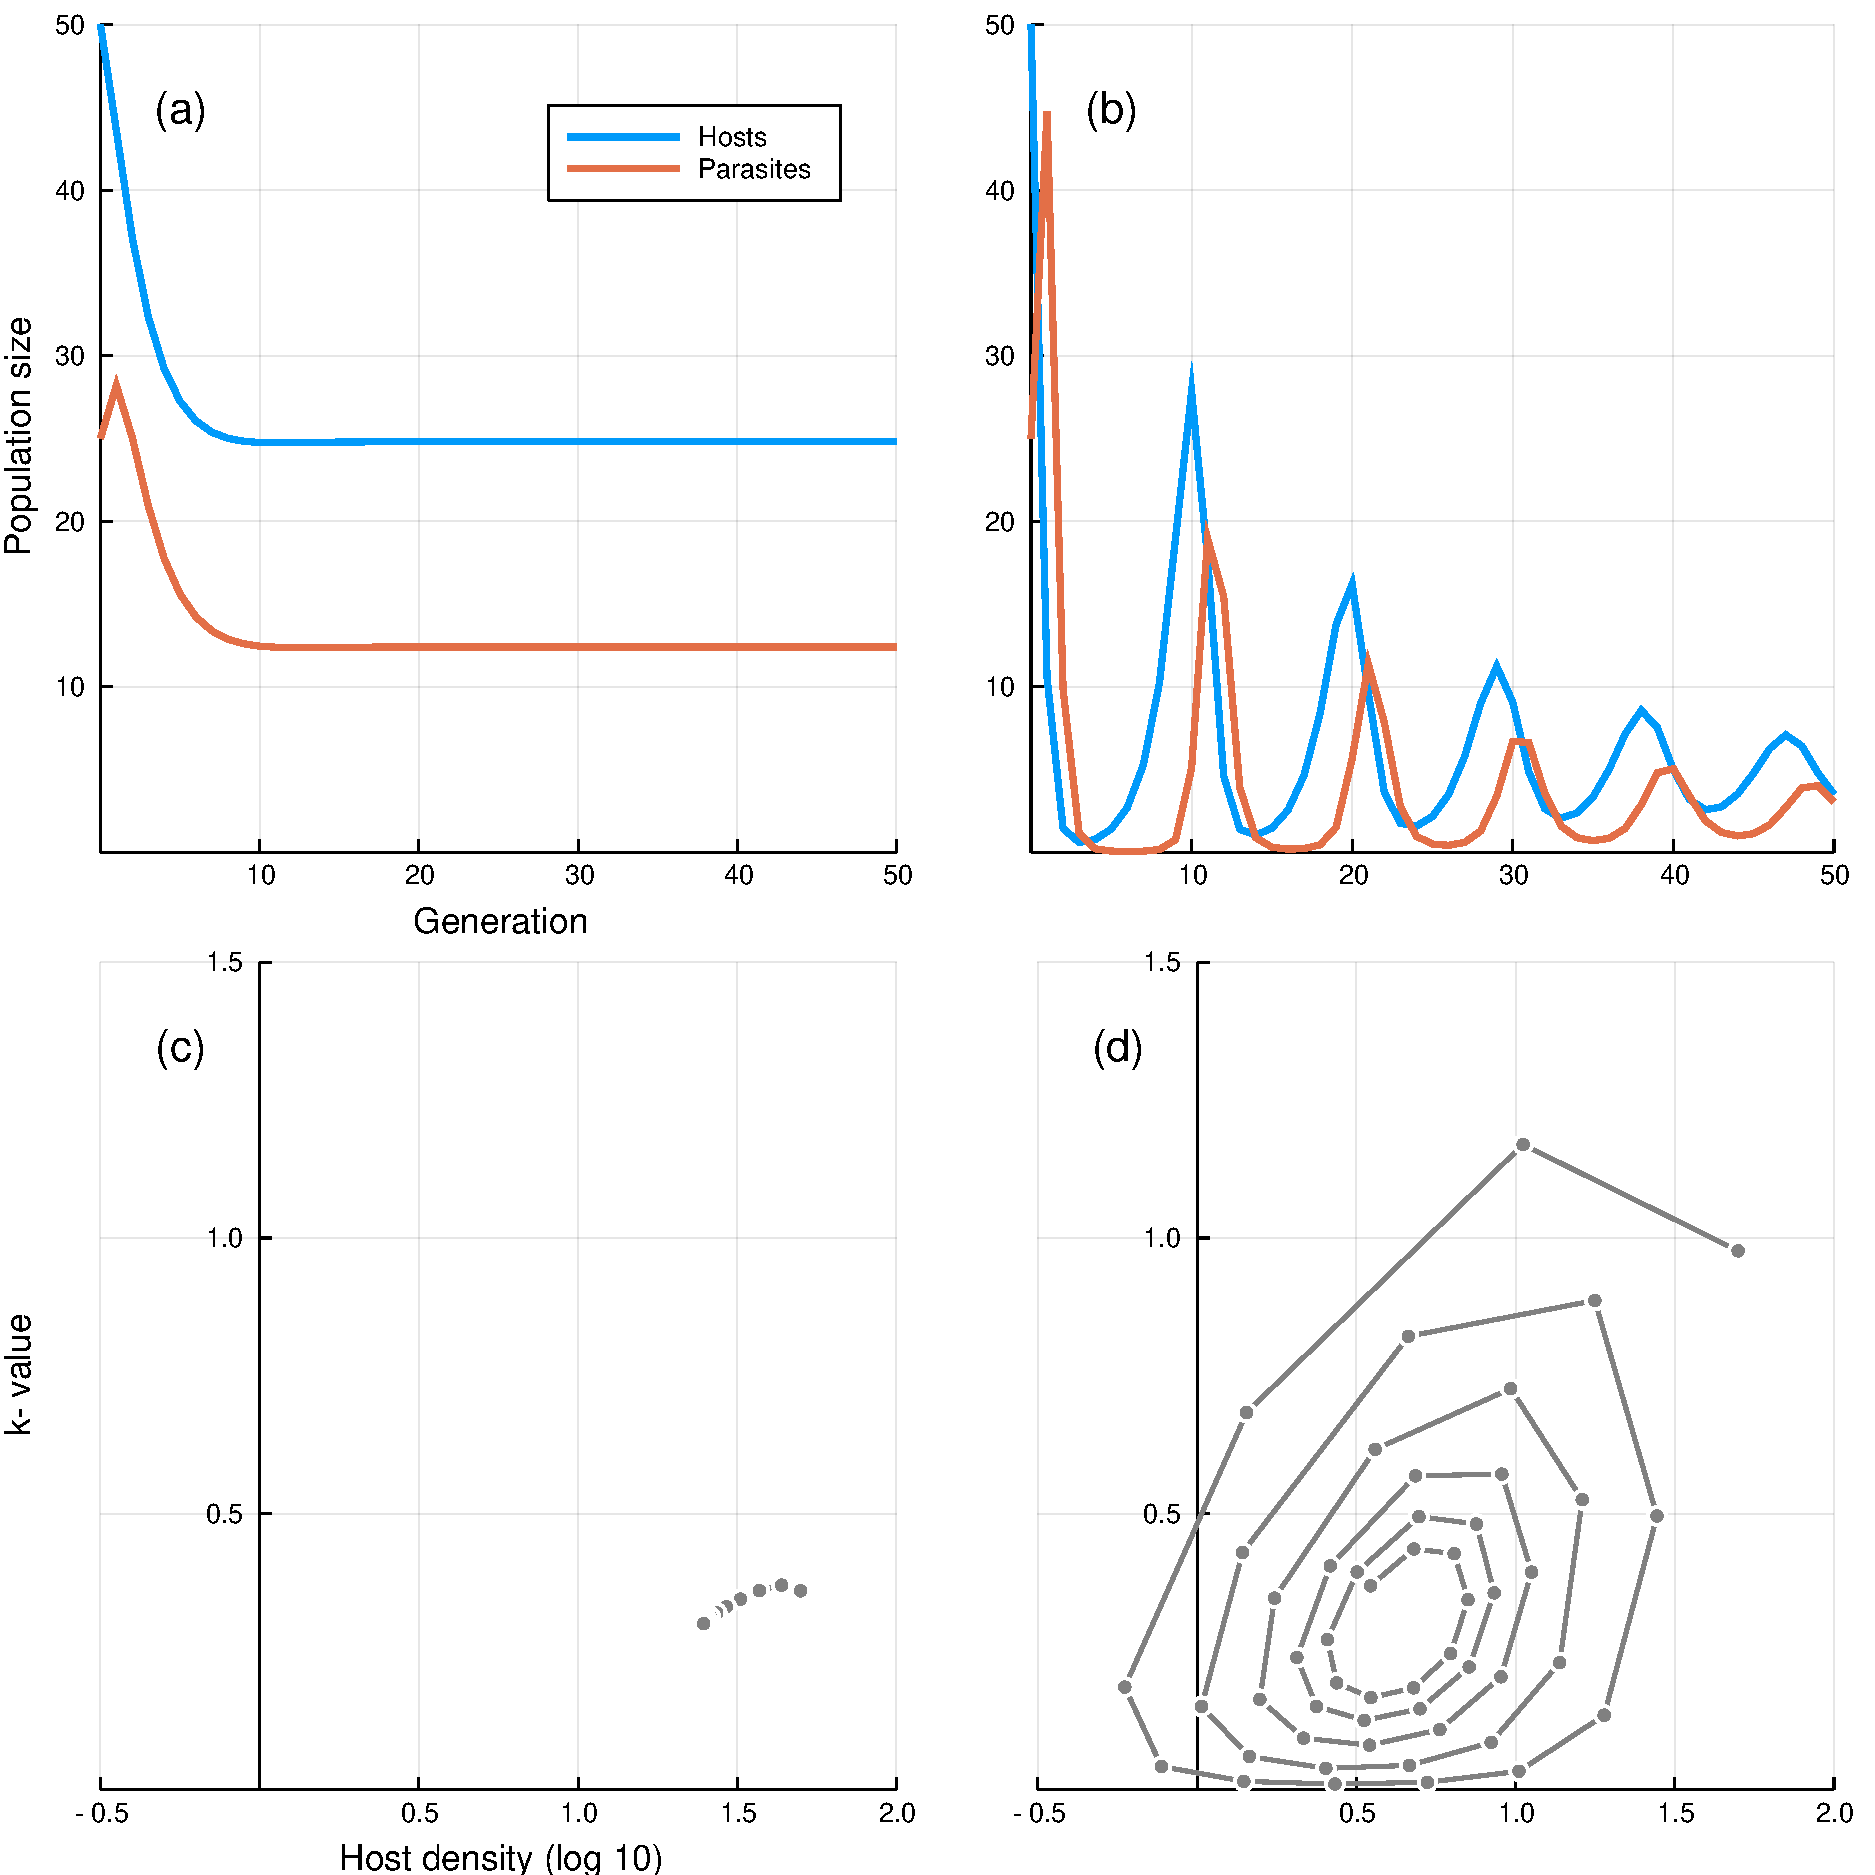
\includegraphics{figures/figure3.pdf}
\caption{(a) and (b) Deterministic simulations of the host and
specialist parasite population dynamics (Eq.1, Eq.2, Eq.3) using two
different level of clumping in the parasitoid attacks: (a) m = 0.2; (b)
m = 0.8. The other parameters used are the same in both (a) and (b): F =
4, D = 0.5, c = 1, a = 0.5 and T\emph{h} = 0. (c) and (d) The
relationship between the mortality caused each generation by parasitism
(k-values) and the log10 host density for the fifty first generations,
linked to (a) and (b) respectively.}\label{fig:figure3}
}
\end{figure}

\begin{figure}
\hypertarget{fig:figure4}{%
\centering
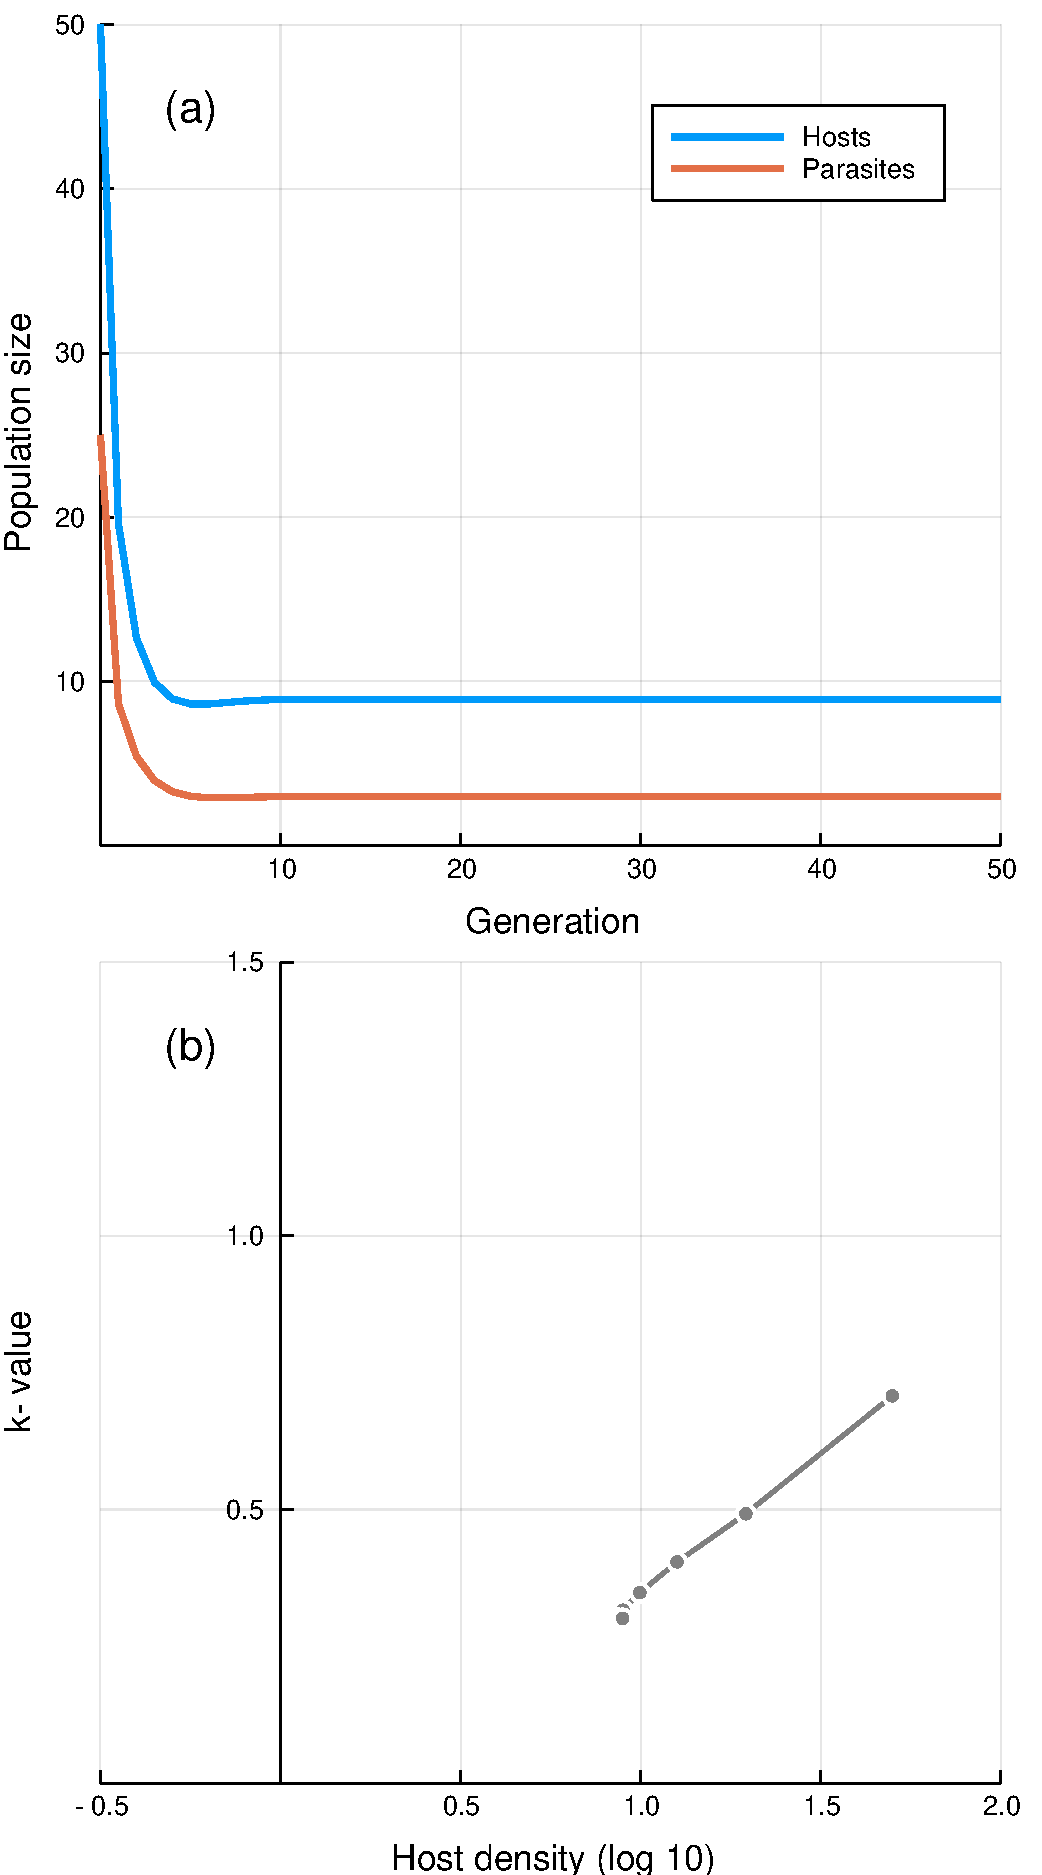
\includegraphics{figures/figure4.pdf}
\caption{(a) Deterministic simulations of the host and generalist
parasite population dynamics (Eq.1, Eq.3, Eq.4) with the following
parameters: F = 4, D = 0.5, h = 10, b = 25, a = 0.5 and T\emph{h} = 0
and m = 0.5. (b) The relationship between the mortality caused each
generation by parasitism (k-values) and the log10 host density for the
fifty first generations of the population dynamics in
(a).}\label{fig:figure4}
}
\end{figure}

\begin{figure}
\hypertarget{fig:figure5}{%
\centering
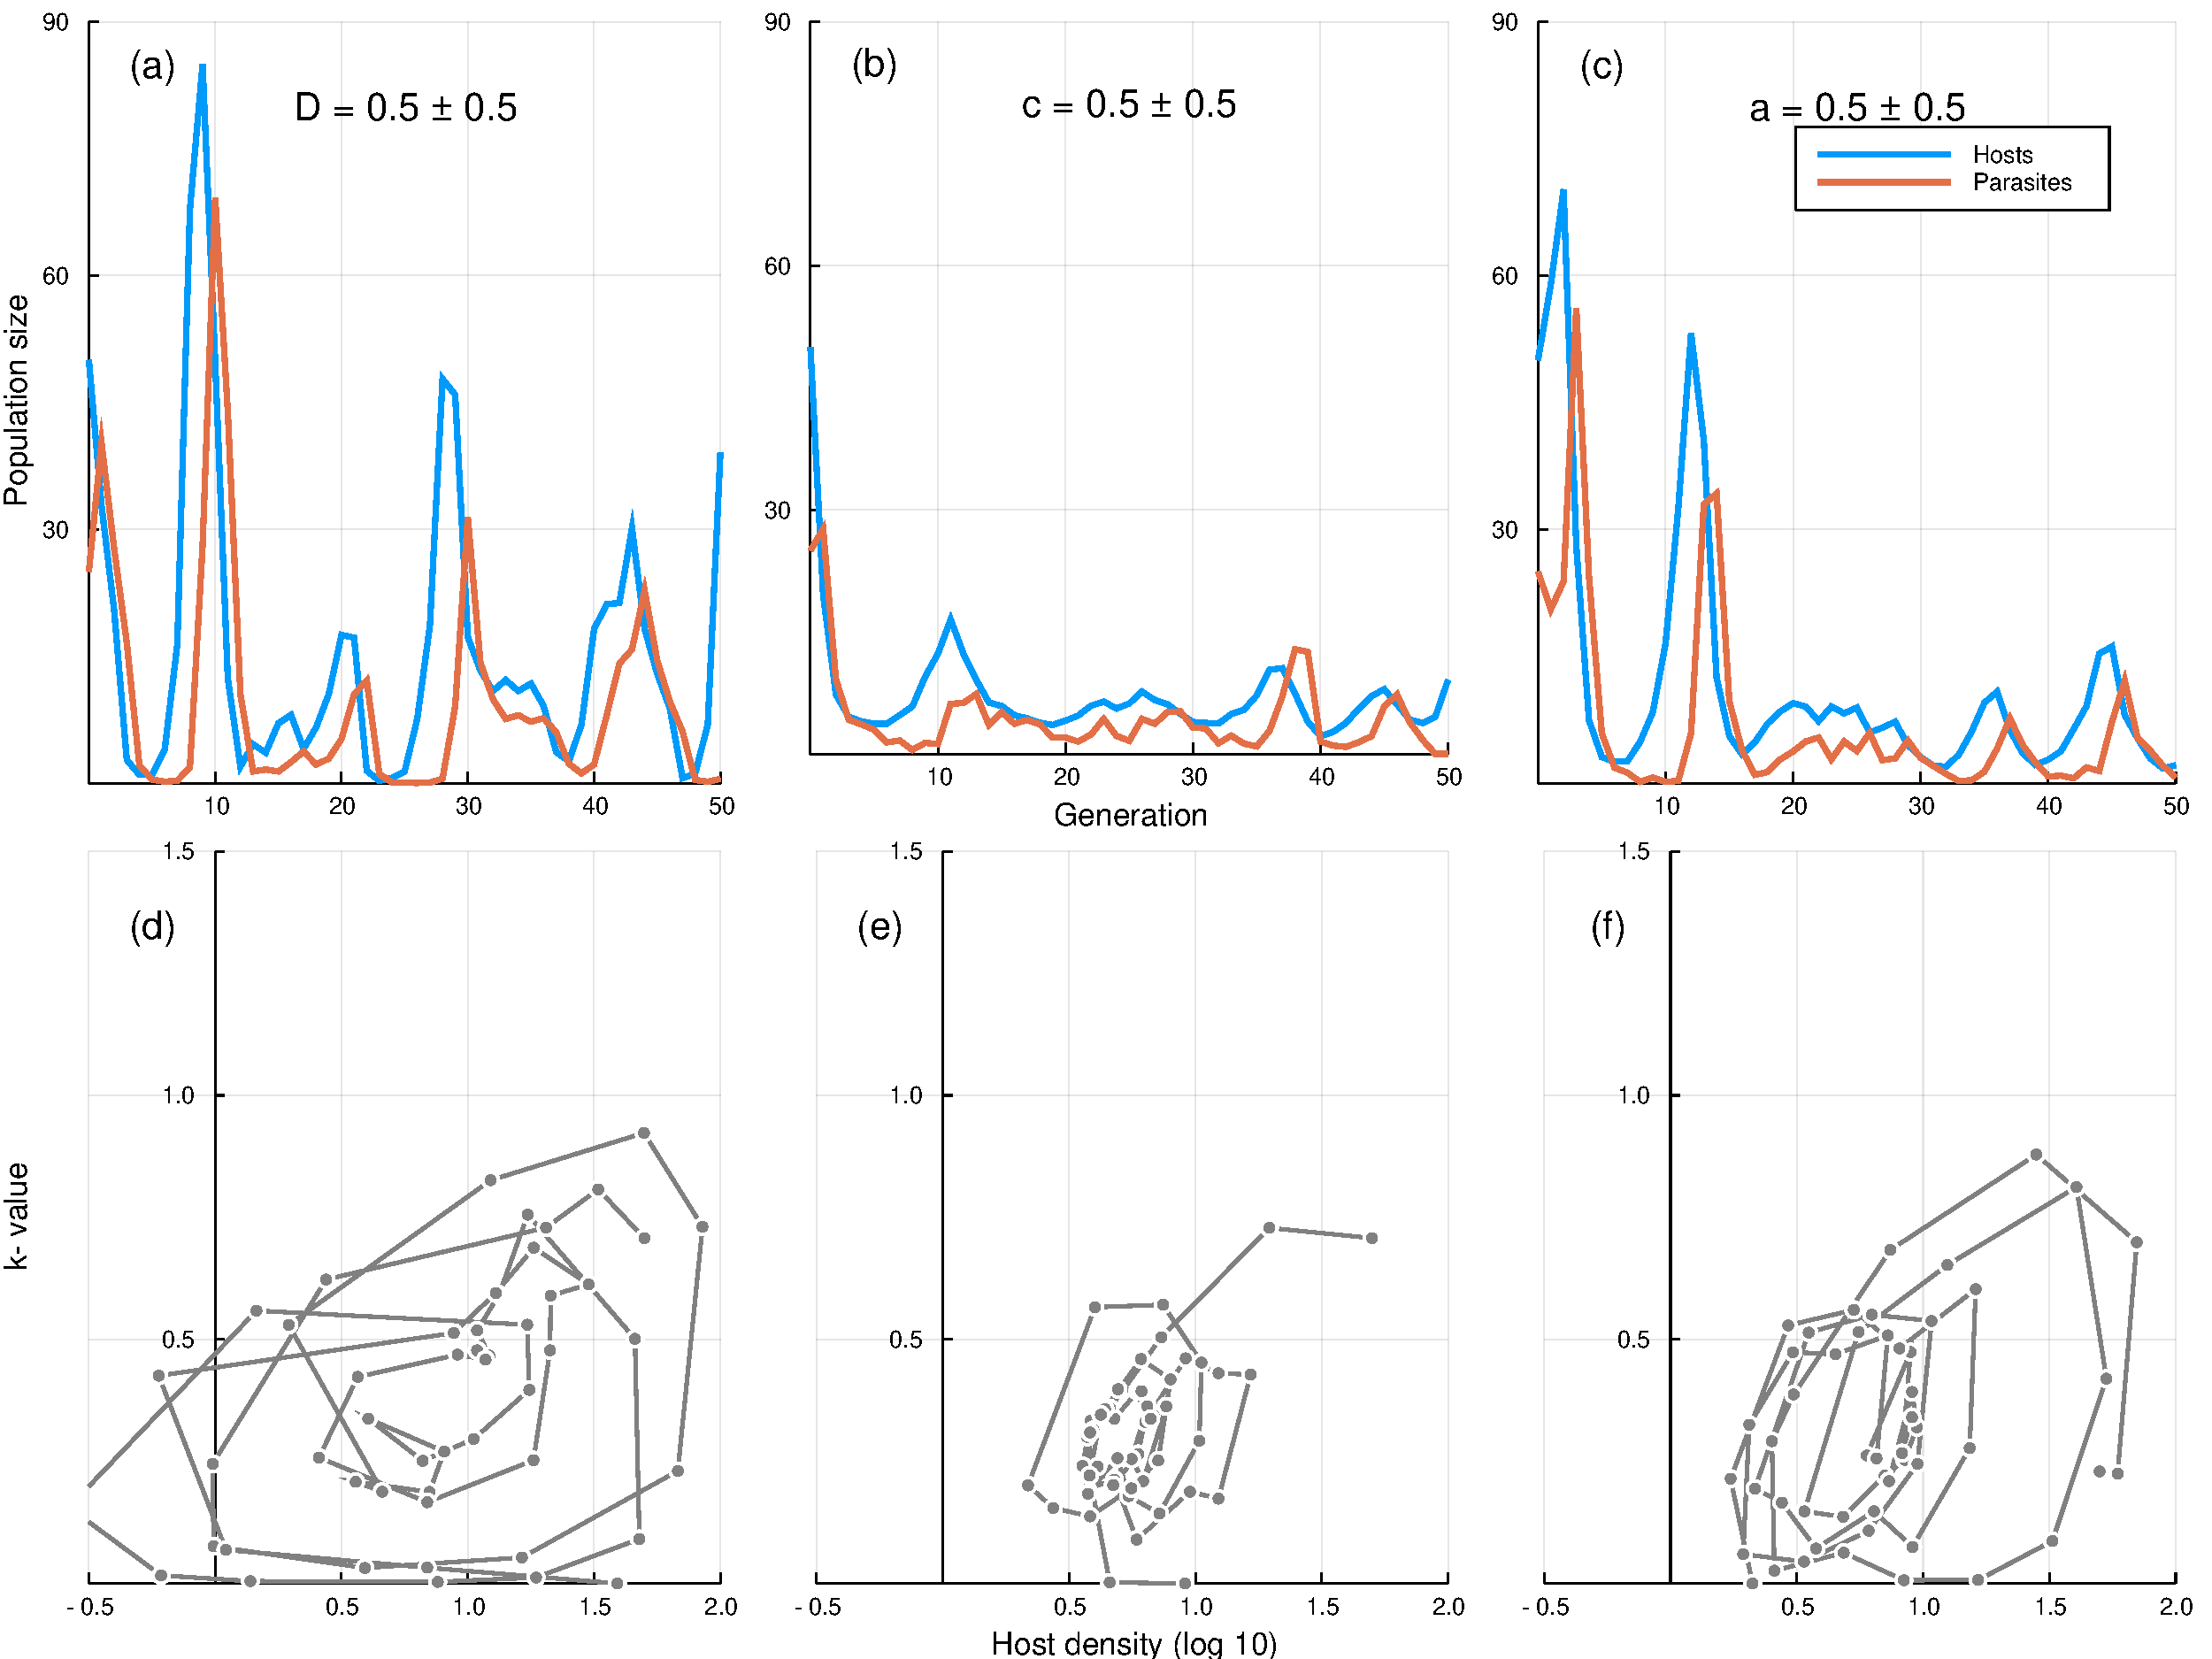
\includegraphics{figures/figure5.pdf}
\caption{(a) - (c) Deterministic simulations of the host and specialist
parasite population dynamics (same as in Figure 3a) except for one
parameter that is treated as a normally distributed stochastic variable:
(a) D = 0.5 ± 0.5, (b) c = 0.5 ± 0.5 and (c) a = 0.5 ± 0.5. The other
parameters are the same as in Figure 3a. (d) - (f) The relationship
between the mortality caused each generation by parasitism (k-values)
and the log10 host density for the fifty first generations, linked to
(a), (b) and (c) respectively. The regression statistics for each
relationship go as follows: (d) \emph{y} = 0.049 + 0.148\emph{x};
\emph{r\^{}2} = 0.564. (e) \emph{y} = 0.082 + 0.113\emph{x};
\emph{r\^{}2} = 0.034. (f) \emph{y} = 0.083 + 0.158\emph{x};
\emph{r\^{}2} = 0.082.}\label{fig:figure5}
}
\end{figure}

\begin{figure}
\hypertarget{fig:figure6}{%
\centering
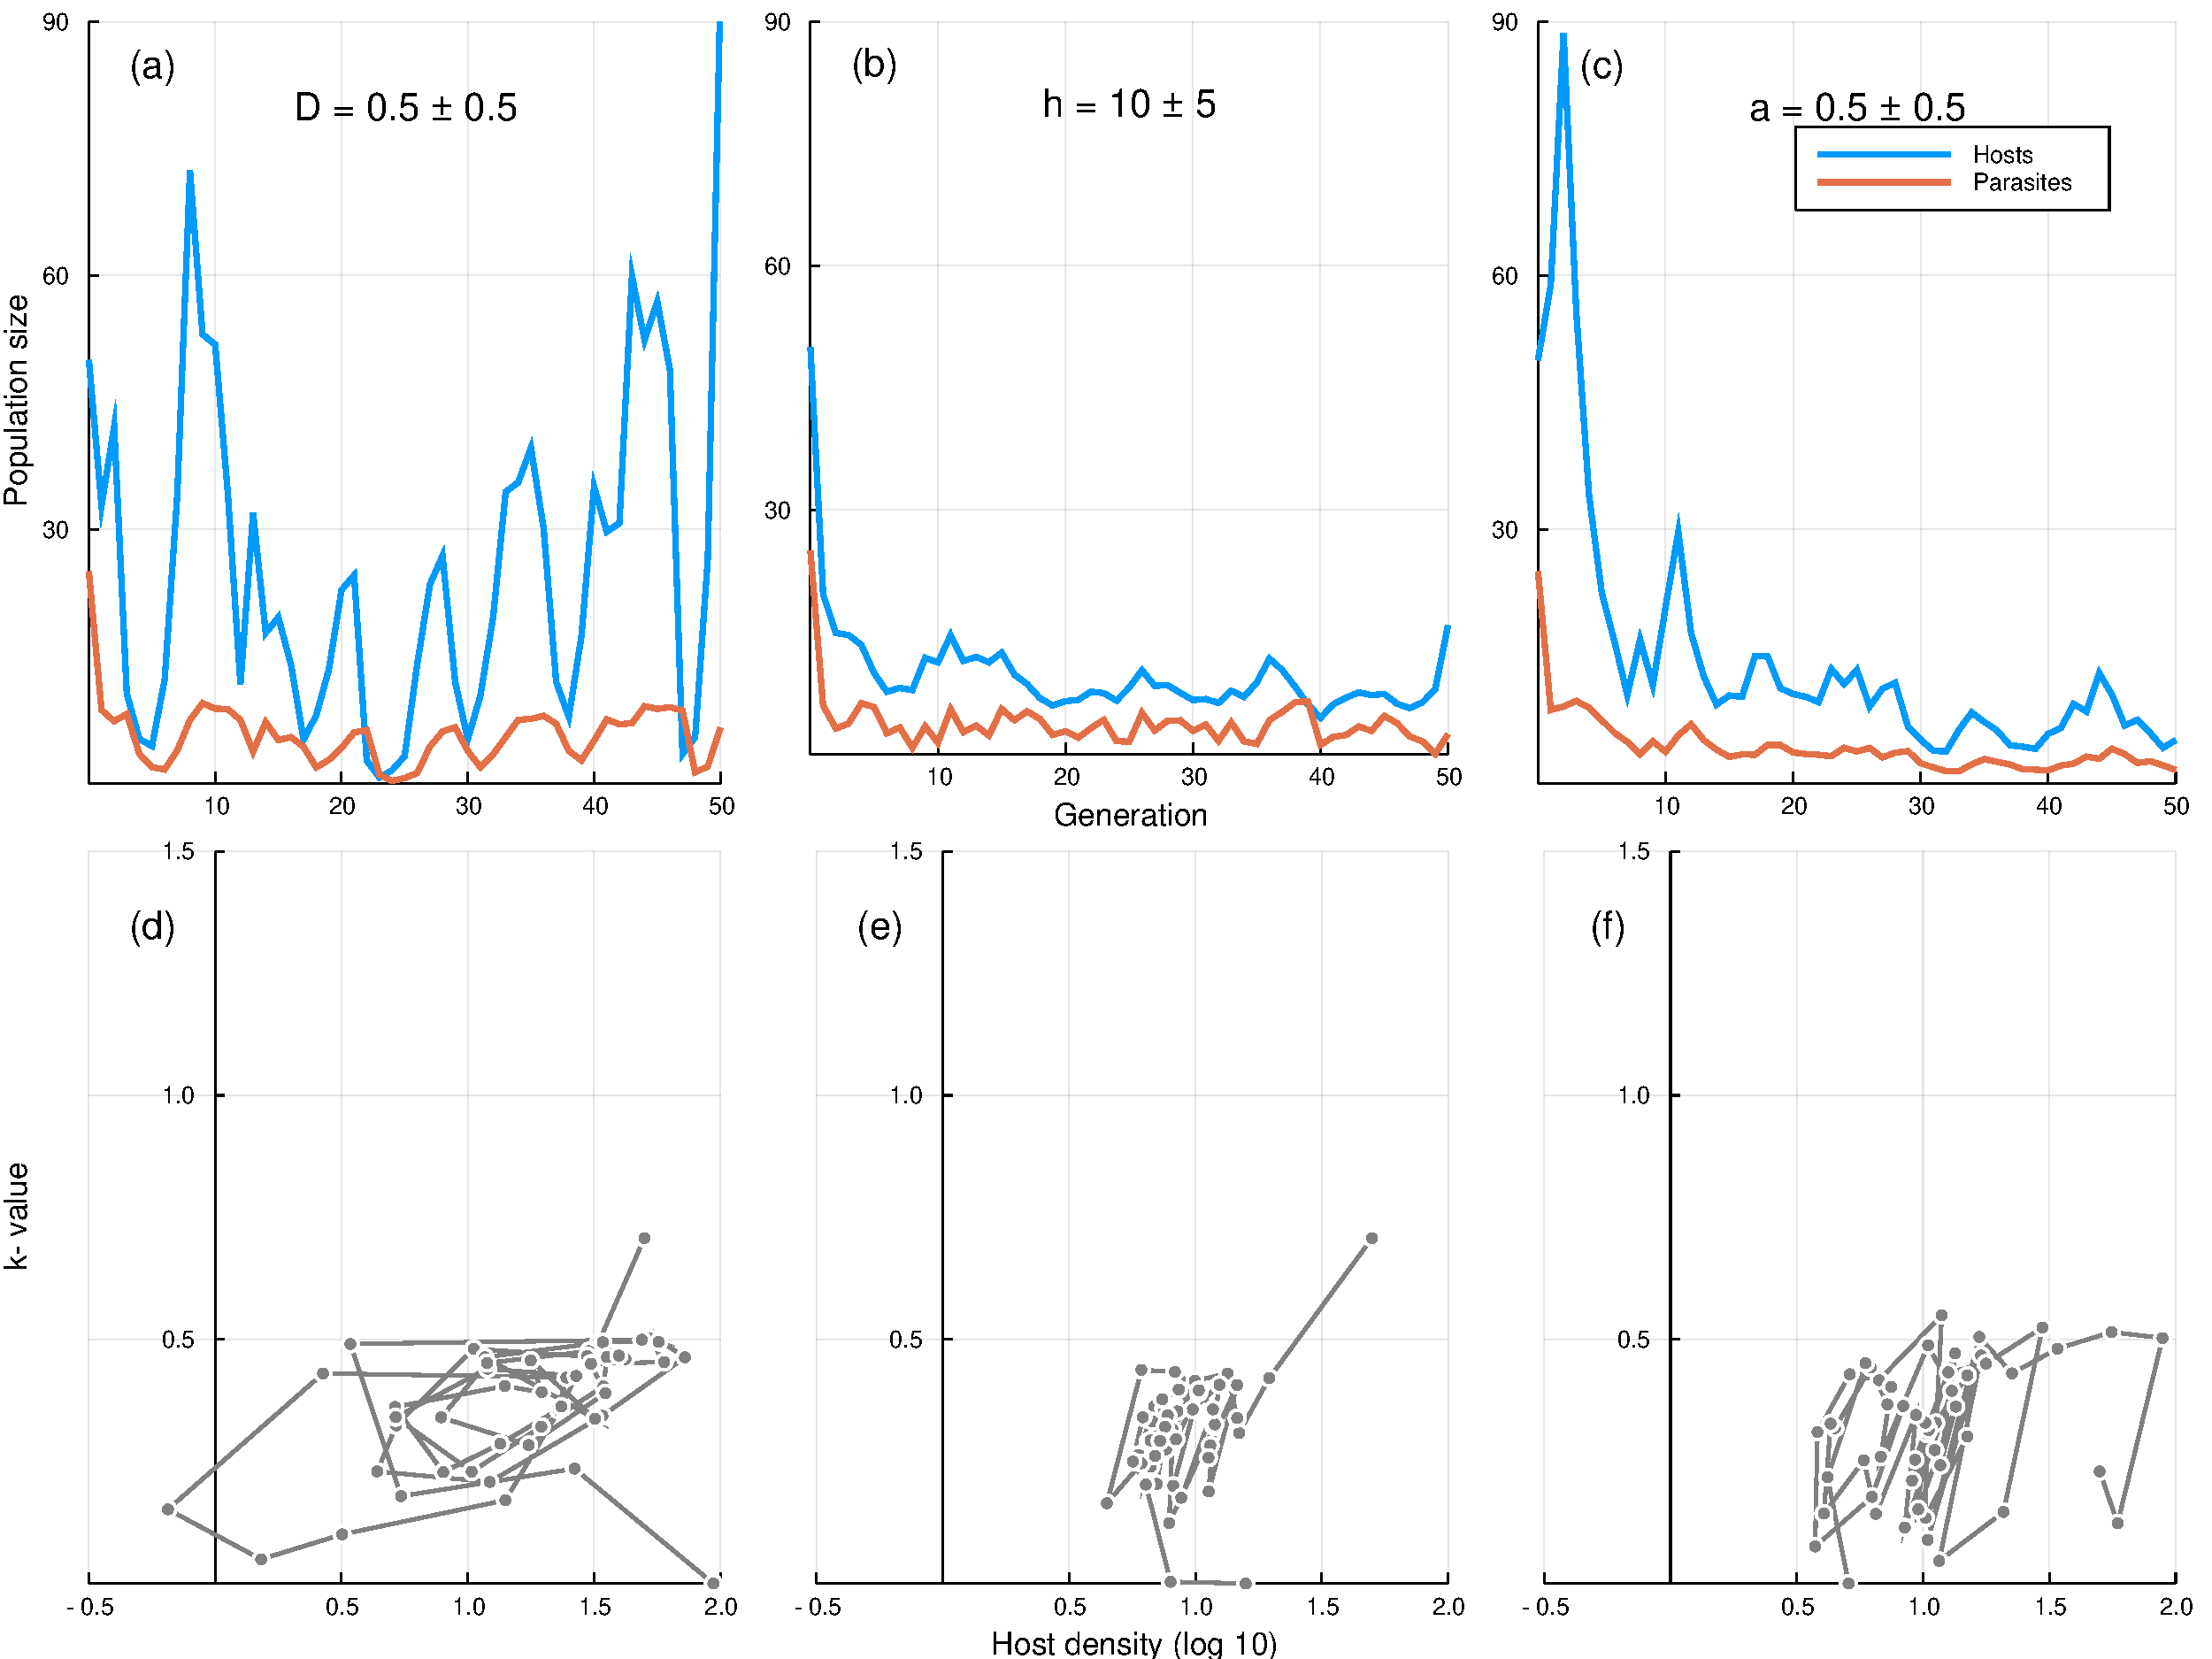
\includegraphics{figures/figure6.pdf}
\caption{(a) - (c) Deterministic simulations of the host and generalist
parasite population dynamics (same as in Figure 4a) except for one
parameter that is treated as a normally distributed stochastic variable:
(a) D = 0.5 ± 0.5, (b) h = 10 ± 5 and (c) a = 0.5 ± 0.5. The other
parameters are the same as in Figure 3a. (d) - (f) The relationship
between the mortality caused each generation by parasitism (k-values)
and the log10 host density for the fifty first generations, linked to
(a), (b) and (c) respectively. The regression statistics for each
relationship go as follows: (d) \emph{y} = 0.111 + 0.174\emph{x};
\emph{r\^{}2} = 0.843. (e) \emph{y} = -0.010 + 0.307\emph{x};
\emph{r\^{}2} = 0.187. (f) \emph{y} = -0.106 + 0.444\emph{x};
\emph{r\^{}2} = 0.262.}\label{fig:figure6}
}
\end{figure}

\begin{figure}
\hypertarget{fig:figure7}{%
\centering
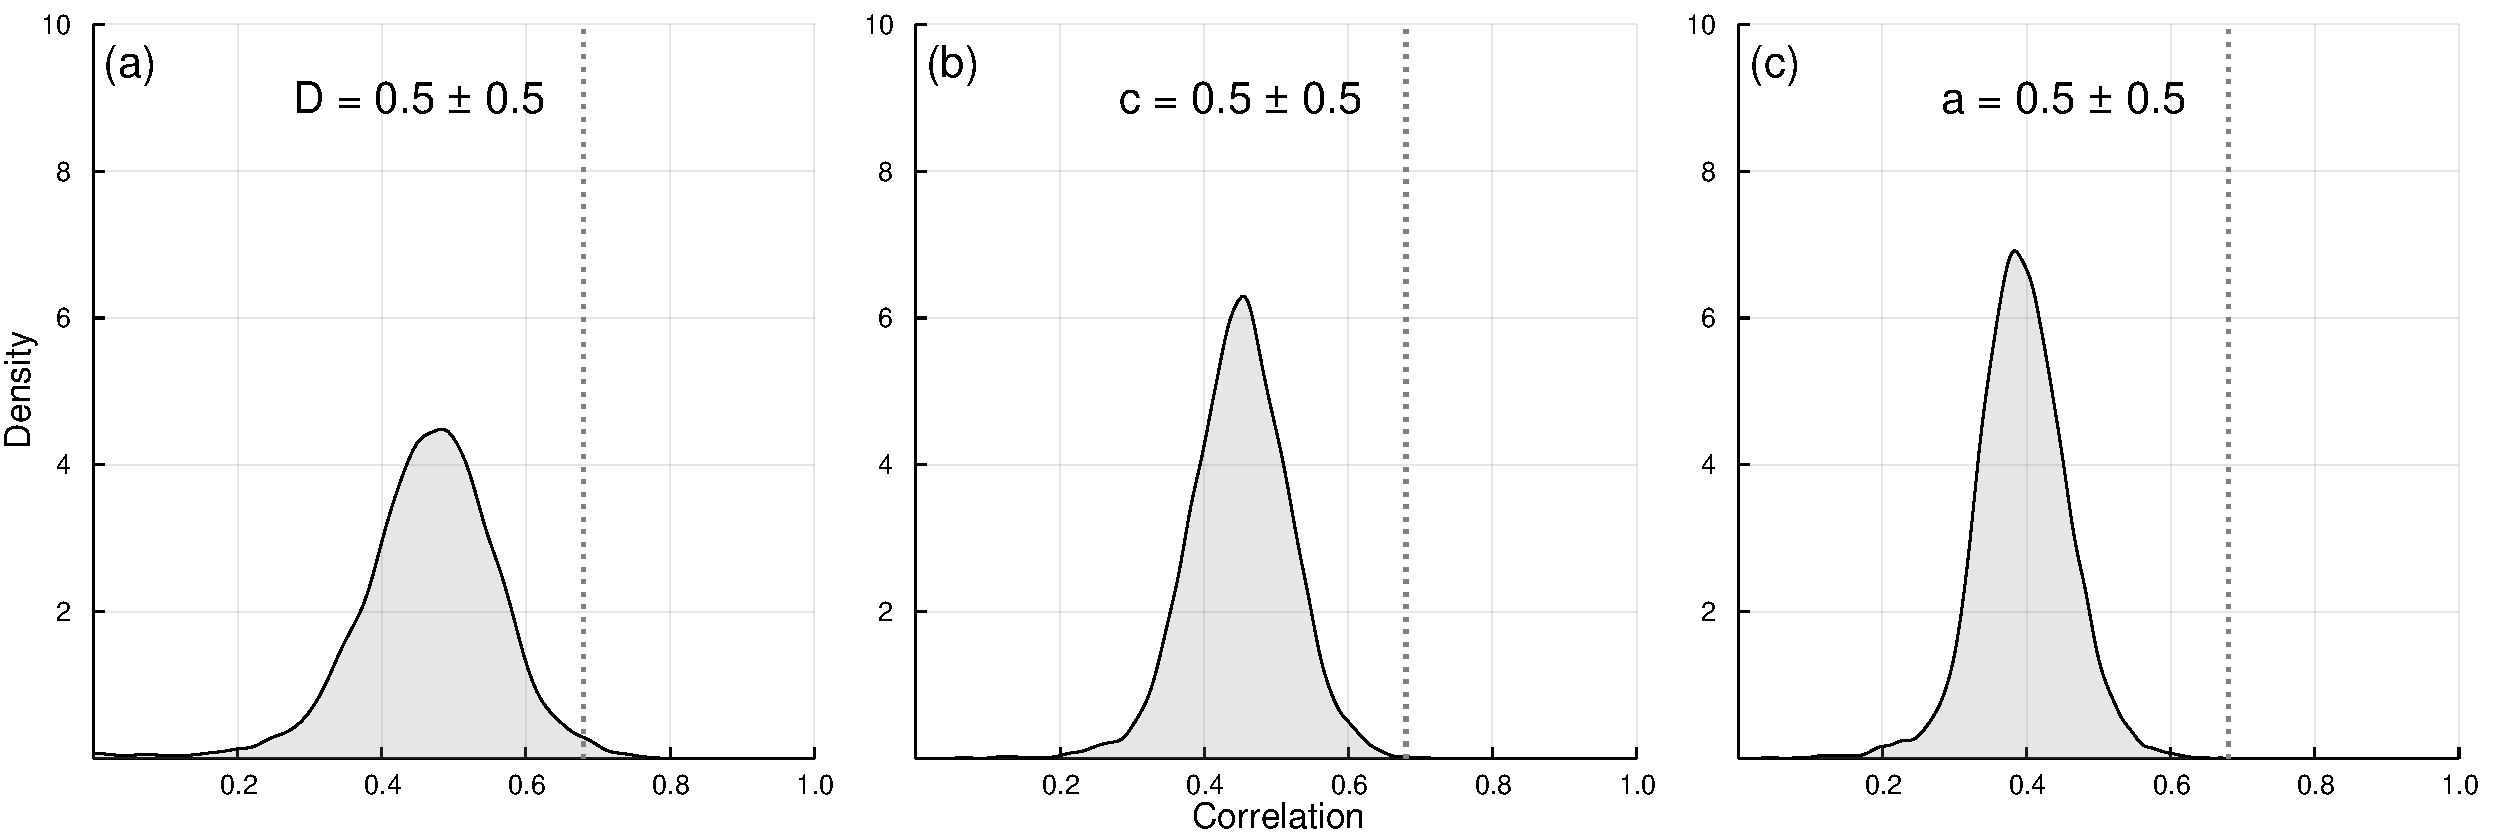
\includegraphics{figures/figure7.pdf}
\caption{(a) - (c) Distribution of the values of correlation coefficient
(\(r\)) obtained for the 5000 simulations done in Figure 5(d) to Figure
5(f) respectively. The dotted line represents the value of \(r\)
obtained in the deterministic model.}\label{fig:figure7}
}
\end{figure}

\begin{figure}
\hypertarget{fig:figure8}{%
\centering
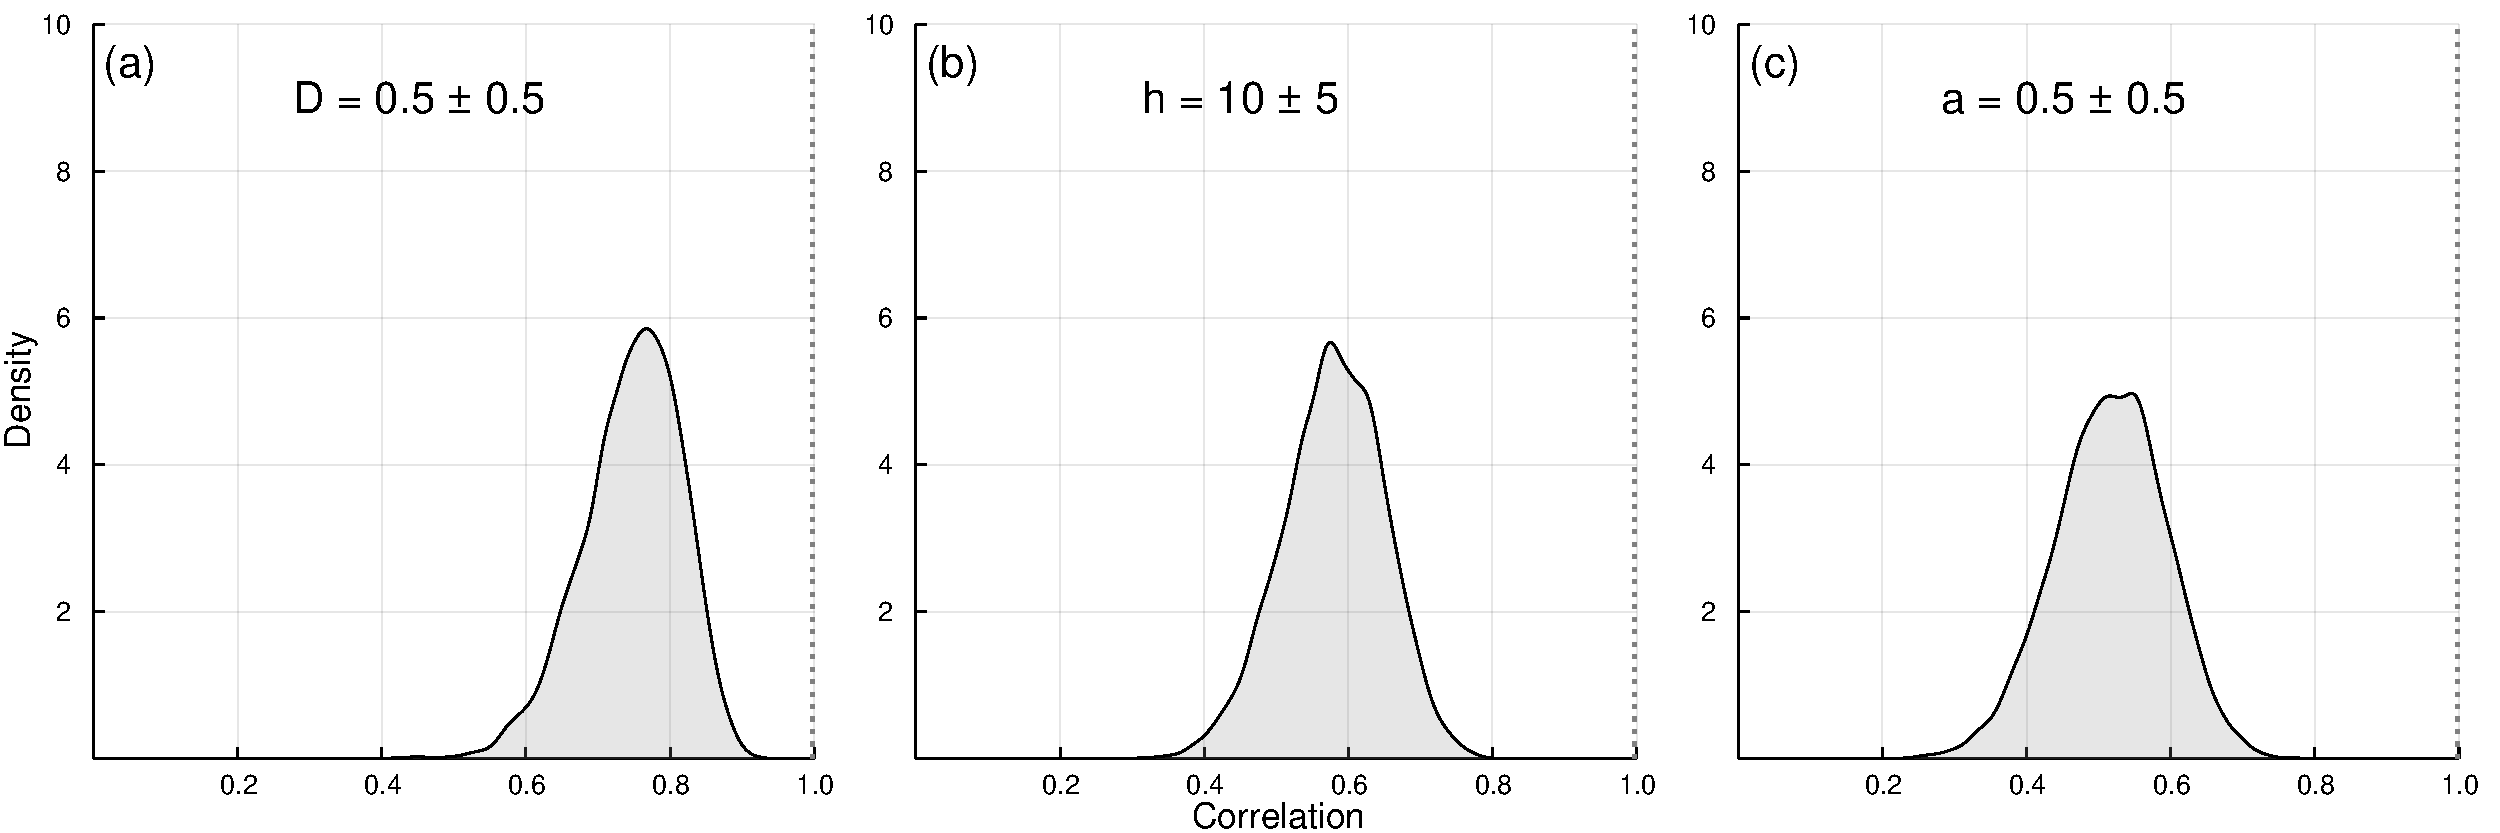
\includegraphics{figures/figure8.pdf}
\caption{(a) - (c) Distribution of the values of correlation coefficient
(\(r\)) obtained for the 5000 simulations done in Figure 6(d) to Figure
6(f), respectively. The dotted line represents the value of \(r\)
obtained in the deterministic model.}\label{fig:figure8}
}
\end{figure}

\begin{figure}
\hypertarget{fig:figure9}{%
\centering
\includegraphics{figures/figure9.pdf}
\caption{(a) Deterministic simulations of the host and generalist
parasite population dynamics (same as in Figure 6b) except that we used
\emph{h} = 5 ± 5. (b) The relationship between the mortality caused each
generation by parasitism (k-values) and the log10 host density for the
fifty first generations, linked to (a). The regression statistics go as
follows: \emph{y} = 0.030 + 0.192\emph{x}; \emph{r\^{}2} =
0.095.}\label{fig:figure9}
}
\end{figure}

{\sffamily \small
  \printbibliography[title=References]
}
\end{document}
